%!TEX root=thesis.tex

\chapter{The User Experience}

% Command - B = compile

\section{Target End-Users Of the Application}

The main end-users of our product are children with ages between 8 and 15 years old. Part of our development strategy was a continuous testing of the platform with representatives of this group age. We have set our testing environment through the workshops in which we have been assisting as tutors. 
We have desiged the platform iteratively based on continuous feedback from our focus groups. We have redesigned features in accordance with free observations of users interacting with our product and with direct feedback from them. \\

The other end-users group of the platform are administrators, which at the moment are represented by the tutors of the workshops. By playing both the role of a tutor and the developer of the application, I had the chance in directly testing the usability myself in the real life context of the product.\\

Consequently, the application has two modes for the two target groups. The profile and the needs of two types of end-users appeal for quite different presentation styles. We focused in designing a user friendly interface for the main target which are the kids, and invested less effort in polishing the administrator panel.	\\

As a central user experience convention, we have kept a minimalistic design for the whole app, both as an aesthetic principle and as a strategy for further future graphics integration.	
In the next subsections of the chapter I will briefly describe what are the main features of each end-users mode.


\section{Typical Usecase for Kids}

\subsection{Experential Learning (Learning by doing): Projects}

Projects Section is a central component of the learning experience on the platform.
The main page of the module displays all projects to users and a searching feature for projects by labeled categories. Projects are briefly presented by a distinctive image and their title. [Figure ~\ref{fig:projects_display}]\\

\begin{figure}
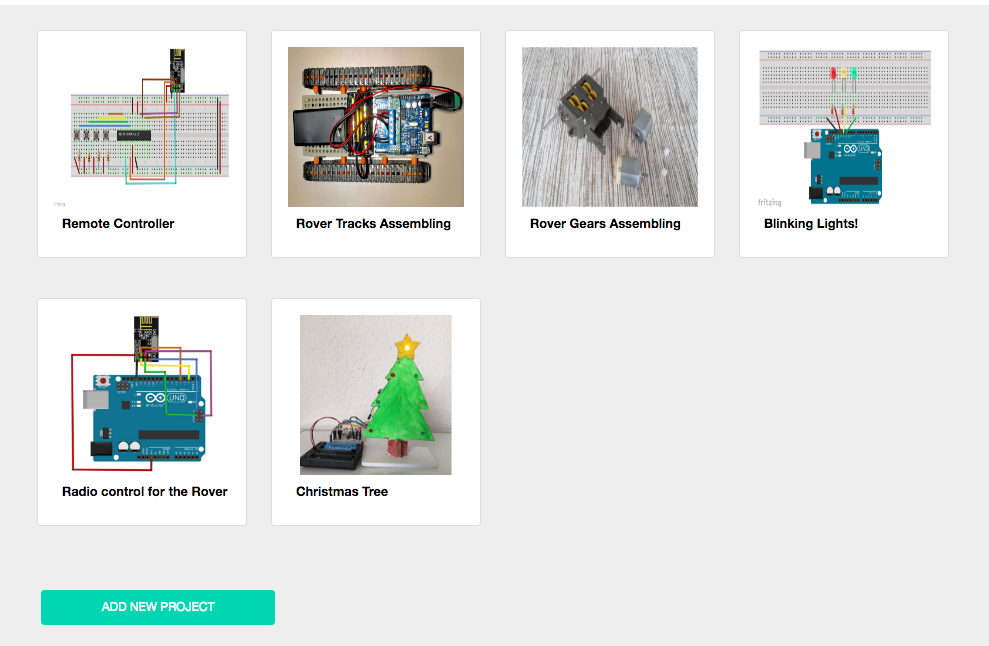
\includegraphics[width=1\linewidth]{images/ui/DisplayProjects.png}
\caption{Main Projects Page - Projects Overview.}
\label{fig:projects_display}
\end{figure}

Users can create and edit a project. The editing mode is currently open to administrators of the platform for putting up and editing teaching materials related to the project: title, description, media resources, a list of needed materials. This mode supports uploading of files (pdf), images (png, jpeg) and videos.
Kids can create projects as well, so that the users become active contributers to the platform. To ensure appropriate content, the data submitted by kids await check-ups and approval from the administrators before getting uploaded on the website.
In the end we want to create an experience where the user is also author and contributor of the platform. \\

\begin{figure}
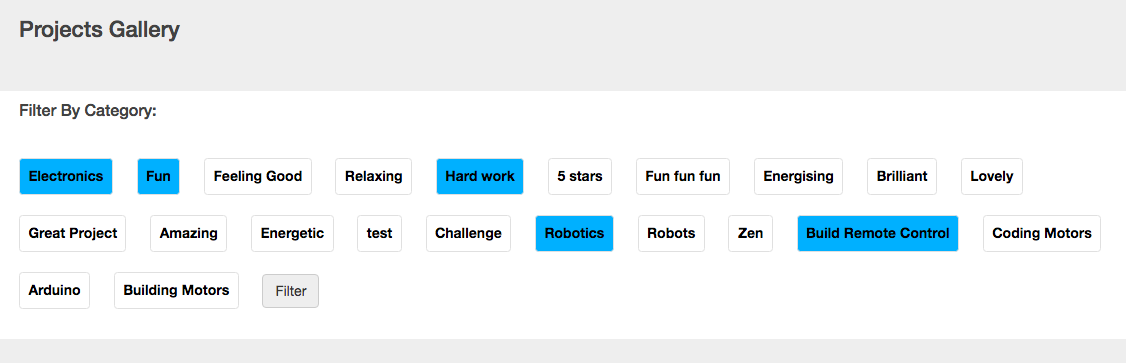
\includegraphics[width=1\linewidth]{images/ui/Labels.png}
\caption{Filtering Category Labels for Projects.}
\label{fig:labels}
\end{figure}

In the project presentation mode, the user finds all details about the current selected project: description, label tags, needed materials or items list (estimated time of completion). The materials list come along with an order and purchase system. Users can check the items they already have and can add to basket for purchase the ones they need. 
Users can leave comments on the page, with questions or any information related to the project. The page includes a stars voting system, where they can rate the project based on a few criterias: functionality, difficulty, fun. (Users will be permitted to vote only after completing the project.)\\

\begin{figure}
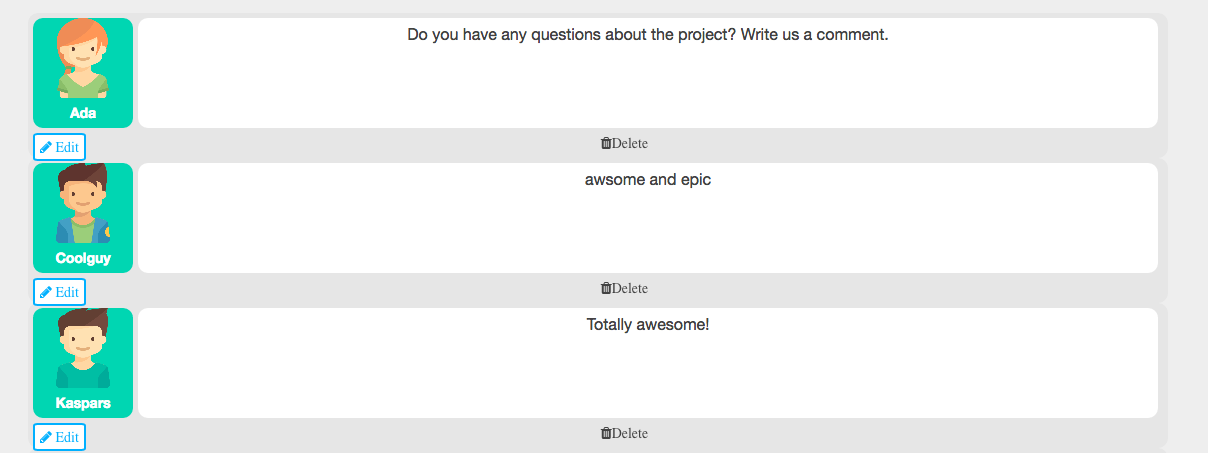
\includegraphics[width=1\linewidth]{images/ui/Comments.png}
\caption{Users Comments System.}
\label{fig:comments}
\end{figure}

\begin{figure}
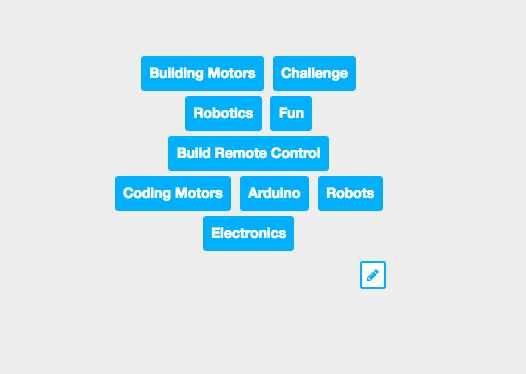
\includegraphics[width=0.5\linewidth]{images/ui/AddLabels.png}
\caption{Add Labels for Project.}
\label{fig:add_labels}
\end{figure}

\begin{figure}
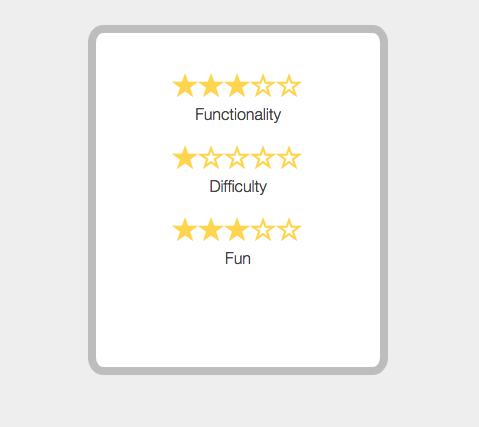
\includegraphics[width=0.5\linewidth]{images/ui/StarsVotingSystem.png}
\caption{Stars Voting System.}
\label{fig:stars_voting_system}
\end{figure}

Each project is split in a number of steps that the user must complete, in order to get rewards such as points and achievements. The user is able to visualize the progress on the tracking progress bar at the top of the steps view. [Figure 2.6] 

\begin{figure}
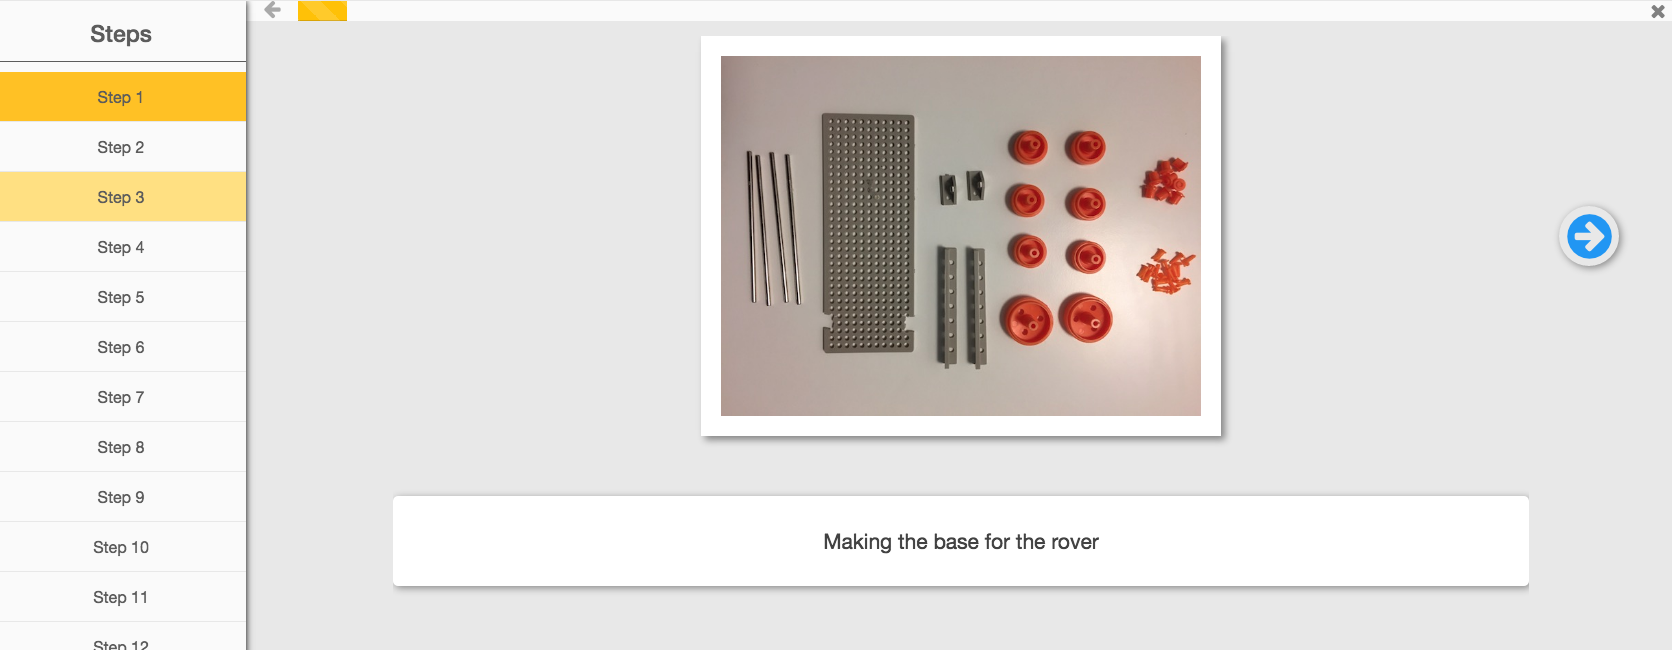
\includegraphics[width=1\linewidth]{images/ui/ProjectSteps.png}
\caption{Project Steps Presentation.}
\label{fig:project_steps}
\end{figure}


\subsection{Learning through Play: Gamification, Rankings, Achievements}

The application is built around a motivational reward system. It uses gamification techniques to transform learning into an engaging and provocative activity. \\

The reward system is represented by achievements and a points system. Achievements have two states: locked and unlocked. They are split in categories, each category standing for certain types of activitis and tasks that the participants can perform. Initially all achievements are locked and they can be activated only when users perform specific actions. The locked state of achievements is visually represented by a grey overlay or background on the achievements (depending on the context where they are displayed). The unlocking of an achievement is marked by a pop up in notifications. The achievements have a general presentation page and can be found also on the user dashboard, where only a maximum of 6 achievements are displayed (always a few unlocked for challenging the user).\\

In the current beta version, there are 2 functional categories of achievements: the the Quiz Achievemnts and the General Achievemnts. The achievements are closely linked to the points system, each coming with a number of points as a reward.\\

\begin{figure}
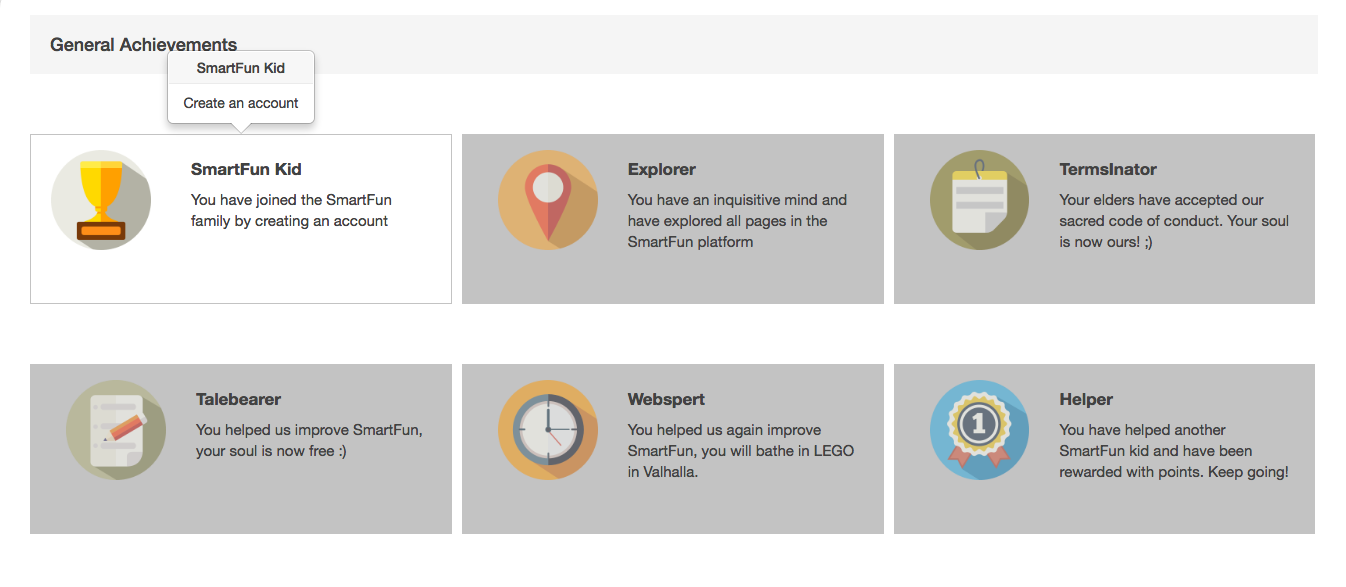
\includegraphics[width=1\linewidth]{images/ui/GeneralAchievements.png}
\caption{General Achievements.}
\label{fig:GeneralAchievements}
\end{figure}

\begin{figure}
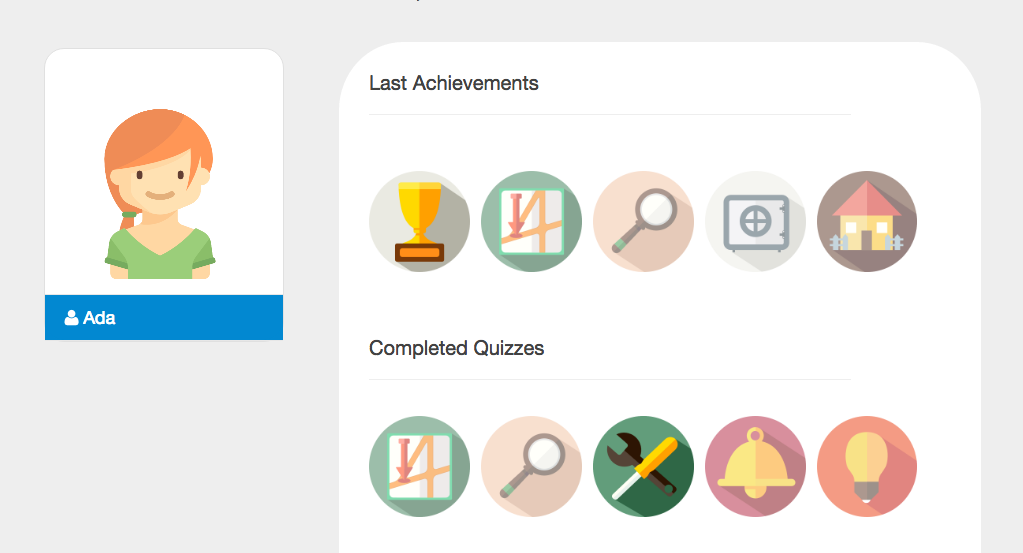
\includegraphics[width=1\linewidth]{images/ui/AchievementsDashboard.png}
\caption{Achievements Display on Dashboard.}
\label{fig:AchievementsDashboard}
\end{figure}

\begin{figure}
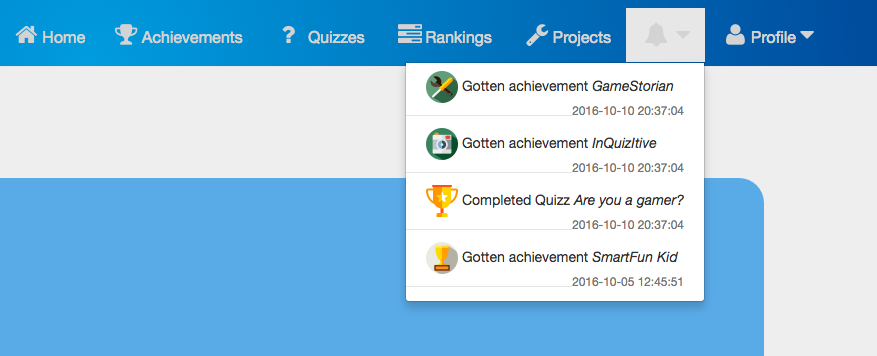
\includegraphics[width=1\linewidth]{images/ui/AchievementsPopUps.png}
\caption{Achievements Notifications.}
\label{fig:AchievementsPopUps}
\end{figure}


The points system is linked to the rankings section which enhance a competitive experience for the users. 
There are 3 types of rankings: \textit{general rankings} - rank individual achievements comparing the performance of all active users; \textit{workshop rankings} - list individual achievements between members of same workshop; \textit{groups rankings} - evaluate collective performance per workshops based on the average points gained by their members. \\

We have intended to design the rankings in a way that stimulates both an individual and collective competitiveness and performance. The rankings per groups targets to boost children spirit of collaboration and feeling of group adherance. \\

During our UX testing sessions with the kids, we have concluded that rankings is the most popular feature of the platform, as kids kept coming back and checking the rankings page many times per session. Rankings was motivating kids in taking more and more quizzes and redoing quizzes for gaining more points.
Based on our UX testing findings, we include on the platform a number of occasions for users to access the rankings: when first logging in on dashboard page, after the completion of a quiz.
\\

\begin{figure}
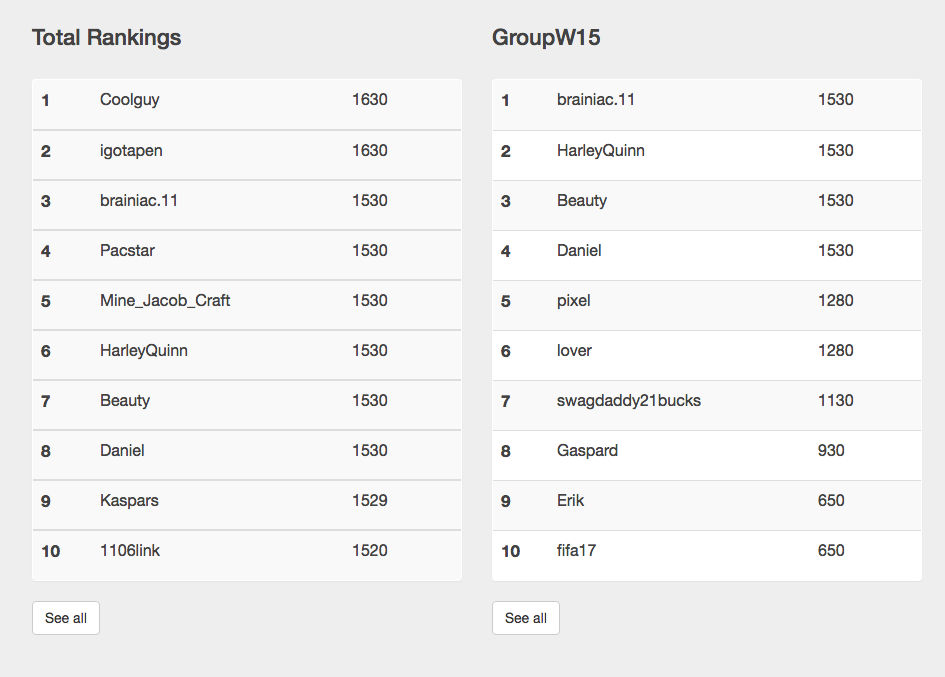
\includegraphics[width=1\linewidth]{images/ui/Rankings.png}
\caption{Ranking System.}
\label{fig:Rankings}
\end{figure}

A central gamification feature intended for the release version will integrate and link together the current gamification elements (achievements and points) by introducing an avatar buiding system. Users will build their avatars trading their achievements and points for items that will constitute parts or accesories of the avatar. We take into consideration adopting a monetary system represented by coins, with an equivalent of points for one coin.

\subsection{Assessment Techniques: Quizzes}

The core feature of the current version, that generates points and unlock achievements are quizzes. Quizzes are linked to workshop themes and to projects and assess users level of mastering a topic. They have multiple choise answers with one or more correct answers.
After completing a quiz, users can evaluate their answers and visualize the wrong answers against the correct ones. 

Users are evaluated by the number of correct answers and by the time of quiz completion. They can redo the quiz to upgrade the completion time, but they can't update their points, which are decided by their first quiz completion. \\

In the future release version, quizzes will be locked by default and will be unlocked only in a logical sequence. 

\begin{figure}
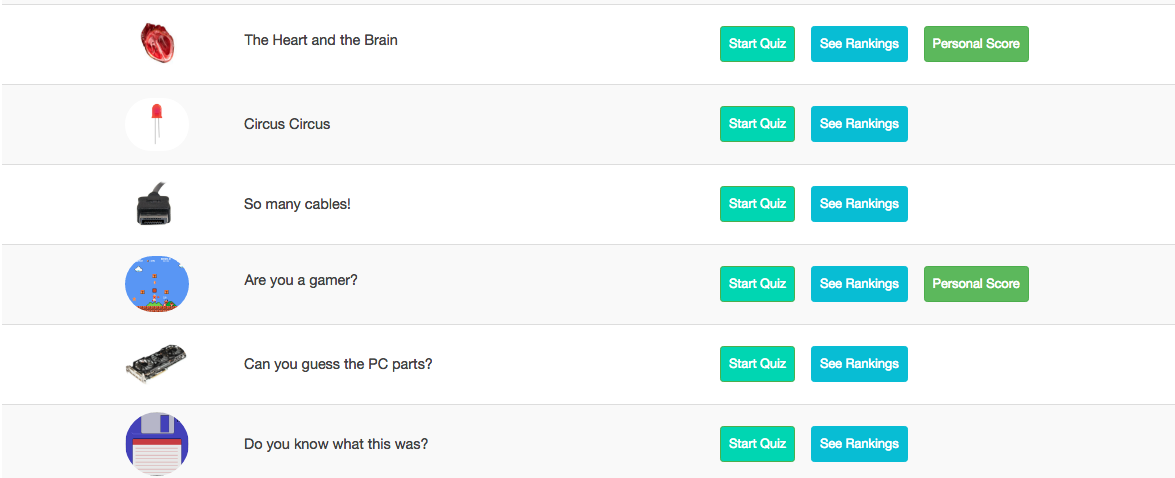
\includegraphics[width=1\linewidth]{images/ui/Quizzes.png}
\caption{Quizzes Overview.}
\label{fig:Quizzes}
\end{figure}

\section{Typical Usecase For Admins}

We have designed the administration panel system in such a way that admins can manage most of the platform content and monitor users activity. From the admin panel, administrators can add and edit content displayed on the platform (quizzes, projects), activate or disable components (the chat system), view and manage users profiles and activity (login history, reset passwords).\\

Each main section on the platform has a correspondent management control in the admin panel.

\begin{figure}
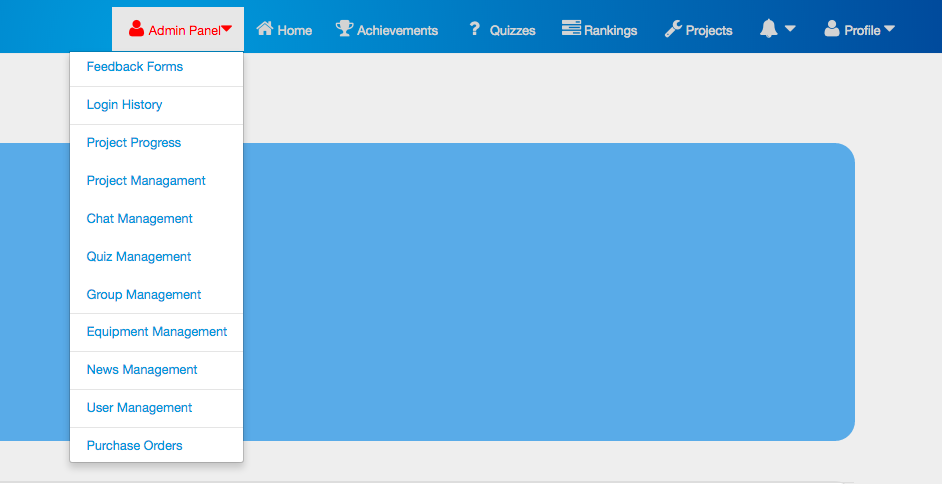
\includegraphics[width=1\linewidth]{images/ui/AdminPanelMenu.png}
\caption{Admin Panel Menu.}
\label{fig:AdminPanelMenu}
\end{figure} 

In the Projects Management section, the admins have an overview of all projects, can edit the display data of the projects or can delete projects from the system. Projects can be
disabled or turned on, meaning admins choose which projects are currently displayed on the projects page. 
Project Management panel includes an users progress tracking feature, which gives admins an overview of the projects started by users and their level of completion progress.
\\

\begin{figure}
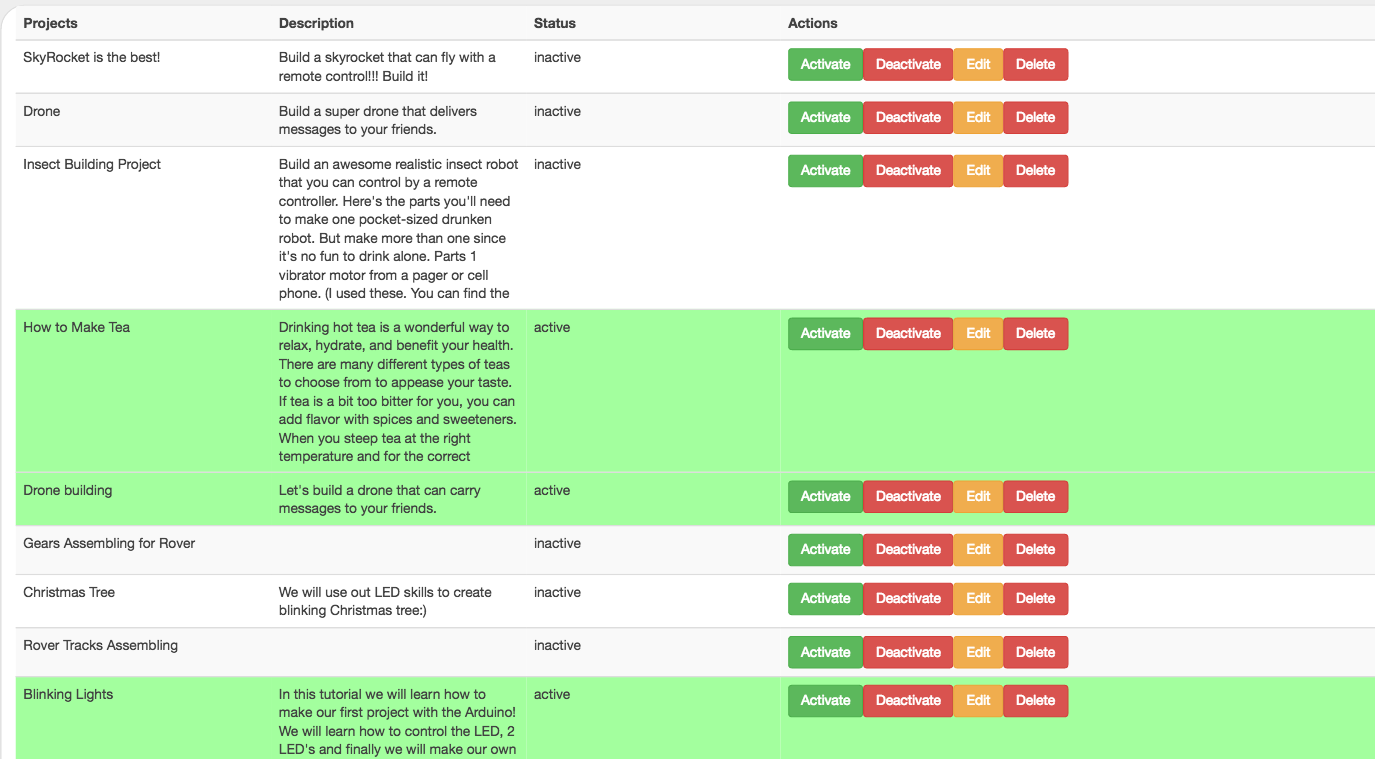
\includegraphics[width=1\linewidth]{images/ui/AdminPanelProjects.png}
\caption{Admin Panel Projects Control.}
\label{fig:AdminPanelProjects}
\end{figure} 

The Quiz Management system allows adding or editing quizzes: uploading images and creating multiple choice answers, setting the correct answer. As it does in projects, the admin system allows the enabling or disabling of quizzes.\\

The profiles and activity of users can be monitored and managed in the User Management panel. The Login History comprises the timestamps of the users having logged in on the application. The Reset Password feature came as a result of a common problem tutors faced in the actual workshops: kids frequently forgetting their credentials. The Group Management is also linked to the real needs of the workshop organisation. We want facilitate the tutors in changing names or adding new workshops, without the need of the developer changing entried in database.

In the Chat Control panel, tutors can disable the chat. We have designed this feature, after chatting during the workshops became a way of distracting kids from working on the projects and paying attention.






















